\documentclass[handout]{beamer} %
\usetheme{CambridgeUS}
\usepackage[latin1]{inputenc}
\usefonttheme{professionalfonts}
\usepackage{times}
\usepackage{graphics}
\usepackage{tikz}
\usepackage{color}
\usepackage{amsmath}
\usepackage{verbatim}
\usepackage{algorithm}
\usepackage{algorithmicx}
\usepackage{booktabs}

\usepackage[style=authoryear]{biblatex}

\addbibresource{references.bib}

% theorem
\BeforeBeginEnvironment{theorem}{
  \setbeamercolor{block title}{fg=red!80!black,bg=gray!10!white}
  \setbeamercolor{block body}{fg=black,bg=white}
}
\AfterEndEnvironment{theorem}{
    \setbeamercolor{block title}{fg=blocktitlefgsave,bg=blocktitlebgsave}
    \setbeamercolor{block body}{fg=blockbodyfgsave,bg=blockbodybgsave}
}

% definition
\BeforeBeginEnvironment{definition}{
  \setbeamercolor{block title}{fg=red!80!black,bg=gray!10!white}
  \setbeamercolor{block body}{fg=black, bg=white}
}
\AfterEndEnvironment{definition}{
    \setbeamercolor{block title}{fg=blocktitlefgsave,bg=blocktitlebgsave}
    \setbeamercolor{block body}{fg=blockbodyfgsave,bg=blockbodybgsave}
}

\renewcommand{\arraystretch}{1.5}

%\setbeamersize{text margin left=0.3mm,text margin right=0.1mm}
\DeclareMathOperator*{\argmin}{argmin}
\DeclareMathOperator*{\argmax}{argmax}
\DeclareMathOperator*{\expit}{expit}
\DeclareMathOperator*{\Cov}{Cov}
\DeclareMathOperator*{\Var}{Var}
\DeclareMathOperator*{\plim}{plim}
\newcommand{\R}{\mathbb{R}}

\usetikzlibrary{shapes,decorations,arrows,calc,arrows.meta,fit,positioning}
\tikzset{
    -Latex,auto,node distance =1 cm and 1 cm,semithick,
    state/.style ={ellipse, draw, minimum width = 0.7 cm},
    point/.style = {circle, draw, inner sep=0.04cm,fill,node contents={}},
    bidirected/.style={Latex-Latex,dashed},
    el/.style = {inner sep=2pt, align=left, sloped}
}

\usepackage{hyperref}
\hypersetup{colorlinks=true, linkcolor=blue, filecolor=magenta, urlcolor=blue}

\author[CL]{Caleb Leedy}
\title[IV]{Instrumental Variables}

\begin{document}

\everymath{\displaystyle}
\setbeamertemplate{title page}[default][colsep=-4bp,rounded=true]
\setbeamertemplate{itemize items}[circle]
\setbeamercolor{block title}{bg=red!50,fg=black}
\frame{\titlepage}

\begin{frame}{Ordinary Least Squares}

\begin{itemize}
    \item<1-> In OLS, we consider the model,

      \begin{equation}\label{eq:ols}
      Y = X\beta + \varepsilon
      \end{equation}

      where $E[\varepsilon \mid X] = 0$ and $X \perp \varepsilon$.
    \item<2-> However, what if $\Cov(X, \varepsilon) \neq 0$?
    \item<3-> We say a variable $X_k$ is \textbf{endogenous} if $\Cov(X_k,
      \varepsilon) \neq 0$.
    \item<3-> A variable $X_k$ is \textbf{exogenous} if $X_k \perp \varepsilon$.
\end{itemize}

\end{frame}

\begin{frame}{Modifying Previous Assumptions}

\begin{itemize}
    \item Last week we discussed the assumptions of the potential outcomes
      framework. One of them was: No Unmeasured Confounders (NUC),

      \[Y(1), Y(0) \perp A \mid X.\]

    \item If a variable $X_k$ is endogenous, then the model does \textit{not} 
      satisfy the NUC condition.
\end{itemize}

\end{frame}

\begin{frame}{Parametric Models}

\begin{itemize}
  \item Consider the following linear model:\footnote{Example taken from
    (\cite{wooldridge2010econometric}).}
      \[y = \beta_0 + \beta_1 x_1 + \beta_2 x_2 + \beta_3 x_3 + \varepsilon\]
      with $x_1, x_2 \perp \varepsilon$ but $x_3 \not\perp \varepsilon$
    \item To estimate $\beta_3$ we need an instrumental variable.
\end{itemize}

\end{frame}

\begin{frame}{Instrumental Variables}

\begin{itemize}
  \item A variable $z_1$ is an \textbf{instrumental variable} (IV) if it
    satisfies:
    \begin{align}
      \Cov(z_1, \varepsilon) &= 0 \label{eq:iv1}\\
      \Cov(z_1, x_3) &\neq 0 \label{eq:iv2}
    \end{align}
  \item This makes sense because we want it to be exogenous with respect to
    Equation~\ref{eq:ols}, yet we need it to influence $x_3$ if we are going to
    measure $\beta_3$.
  \item Note, that Equation~\ref{eq:iv1} \textit{cannot} be tested but
    Equation~\ref{eq:iv2} can and should be tested.
\end{itemize}

\end{frame}

\begin{frame}{Graphical Model}

  \begin{center}
  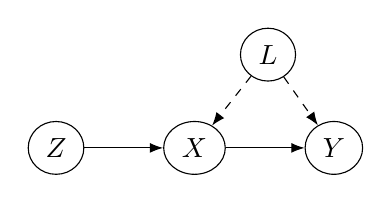
\begin{tikzpicture}
    \node[state] (1) {$Z$};
    \node[state] (2) [right =of 1] {$X$};
    \node[state] (3) [right =of 2] {$Y$};
    \node[state] (4) [above right =of 2,xshift=-0.6cm,yshift=-0.3cm] {$L$};

    \path (1) edge node[above] {} (2);
    \path (2) edge node[above] {} (3);
    \path[dashed] (4) edge node[above] {} (3);
    \path[dashed] (4) edge node[above] {} (2);
  \end{tikzpicture}
  \end{center}

\end{frame}

\begin{frame}{Graphical Model}

  \begin{center}
  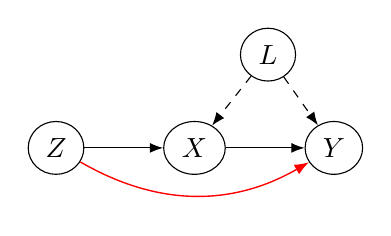
\begin{tikzpicture}
    \node[state] (1) {$Z$};
    \node[state] (2) [right =of 1] {$X$};
    \node[state] (3) [right =of 2] {$Y$};
    \node[state] (4) [above right =of 2,xshift=-0.6cm,yshift=-0.3cm] {$L$};

    \path (1) edge node[above] {} (2);
    \path (2) edge node[above] {} (3);
    \path[dashed] (4) edge node[above] {} (3);
    \path[dashed] (4) edge node[above] {} (2);
    \path[red,line width=0.5] (1) edge[bend right=30] (3);
  \end{tikzpicture}
  \end{center}

\end{frame}

\begin{frame}{Reduced Form Equations}

\begin{itemize}
    \item When we have an instrument $z_1$, we can estimate:
      \begin{align*}
        \hat x_3 &= \hat \gamma_0 + \hat \gamma_1 x_1 + \hat \gamma_2 x_2 
          + \hat \theta z_1\\
        \hat y &= \hat \beta_0 + \hat \beta_1 x_1 + \hat \beta_2 x_2 + \hat
        \beta_3 \hat x_3
      \end{align*}
    \item This framework is called \textbf{two-stage least squares} (2SLS).
    \item This can be generalized to have $K$ exogenous $x_i$ variables and $L$
      instruments $z_j$.
\end{itemize}

\end{frame}

\begin{frame}{Identification}

\begin{itemize}
    \item Then the IV solves the identification problem.
    \item Let $z = (x_1, x_2, z_1)$.
    \item Equation~\ref{eq:iv1} implies that $E[z' \varepsilon] = 0$.
    \item The normal equations for the IV estimator are:
      \[E[z'x]\beta = E[z'y].\]
    \item This has a unique solution if $E[z'x]$ has full rank, which happens if
      Equation~\ref{eq:iv2} is satisfied.
\end{itemize}

\end{frame}

\begin{frame}{Results for 2SLS}

Under regularity conditions, 2SLS is
\begin{itemize}
  \item consistent,
  \item asymptotically normal, and 
  \item asymptotically efficient.
\end{itemize}

  See (\cite{wooldridge2010econometric}), Chapter 5 for these proofs.

\end{frame}

\begin{frame}{Problems with IVs}

  \begin{itemize}
    \item<2-> Bias
    \item<3-> Weak instruments: In the linear model,
      \[\plim \hat \beta_3 = \beta_3 + \frac{\Cov(z_1, \varepsilon)}{\Cov(z_1,
      x_3)}.\]
  \end{itemize}
  
\end{frame}

\begin{frame}{Causal Models with No Unconfoundedness}

  \begin{itemize}
    \item Suppose that we have the model,\footnote{The rest of the slides were
      based off of Stefan Wager's S361 Causal Inference Notes
      (\cite{wager2020stats}).}
      \[Y_i(a) = Y_i(0) + \tau a_i.\]
      % This uses SUTVA assumption to express the observation as a function of
      % potential outcomes.
      We can also express this as 
      \[Y_i = \alpha + A_i \tau + \varepsilon_i\]
    \item We do \textit{not} use the NUC. So 
      \[Y(1), Y(0) \perp A \mid X.\]
    \item Notice that OLS does not work because
      \[\tau_{OLS} = \frac{\Cov(Y_i, A_i)}{\Var{A_i}} = 
      \frac{\Cov(\tau A_i + \varepsilon, A_i)}{\Var{A_i}} =
      \tau + 
      \frac{\Cov(\varepsilon, A_i)}{\Var{A_i}}\]
  \end{itemize}
  
\end{frame}

\begin{frame}{Causal Models with IVs}

  \begin{itemize}
    \item<1-> We can add an instrument and have something similar to 2SLS,

      \begin{align*}
        Y_i &= \alpha + A_i \tau + \varepsilon_i \\
        A_i &= Z_i \gamma + \eta_i \qquad \varepsilon_i \perp Z_i.
      \end{align*}
    \item<2-> Then
      \[\Cov(Y_i, Z_i) = \Cov(A_i \tau + \varepsilon_i, Z_i) = \tau \Cov(A_i,
      Z_i).\]
    \item<3-> Hence,
      \[\tau = \frac{\Cov{(Y_i, Z_i)}}{\Cov(A_i, Z_i)}.\]
  \end{itemize}
  
\end{frame}

\begin{frame}{Optimal Instruments}

  \begin{itemize}
    \item If $Z$ is a $d$-dimensional vector then we have
      \[\tau = \frac{\Cov{(Y_i, w(Z_i))}}{\Cov(A_i, w(Z_i))}\]
      where $w: \R^d \to \R$.
    \item The optimal choice of $w(\cdot)$ that minimizes the variance of
      $\tau$, is
      \[w^*(Z) \propto E[A \mid Z].\]
  \end{itemize}
  
\end{frame}

\begin{frame}{Estimation}

  The previous slide suggests the following estimation strategy:
  \begin{itemize}
    \item[1.] Estimate $\hat w(\cdot) = E[A \mid Z]$ nonparametrically, and then
    \item[2.] Estimate the covariances using $\hat w$,
      \[\hat \tau = 
      \frac{\hat \Cov{(Y_i, \hat w(Z_i))}}{\hat \Cov(A_i, \hat w(Z_i))}\]
  \end{itemize}

  However, this can fail from overfitting with weak instruments.
  
\end{frame}

\begin{frame}{Cross Fitting}

  A better strategy is to use cross-fitting, and solve
  \[\hat \tau = 
  \frac{\hat \Cov{(Y_i, \hat w^{k(-i)}(Z_i))}}{
    \hat \Cov(A_i, \hat w^{k(-i)}(Z_i))}\]

  where $\hat w^{k(-i)}$ is the estimation of $\hat w$ on the $k$-th fold in
  which element $i$ is missing.
  
\end{frame}

\begin{frame}{Extension to Nonparametric Regression}

  \begin{itemize}
    \item Suppose we have the model:
      \[Y_i = g(A_i) + \varepsilon_i, \quad Z_i \perp \varepsilon_i\]
    \item Then,
      \[E[Y_i \mid Z_i] = \int g(a) f(a \mid z) da.\]
    \item This can be estimated using basis splines (or other nonparametric
      techniques).
  \end{itemize}
  
\end{frame}

\begin{frame}{Local Average Treatment Effects}

  \begin{itemize}
    \item Consider the model:

    \begin{align*}
      Y_i &= \alpha + \tau A_i + \varepsilon_i \\
      A_i &= \gamma Z_i + \eta_i \quad Z_i \perp \varepsilon_i.
    \end{align*}

    \item Then we can identify $\tau$ with

      \begin{align*}
        \tau &= \frac{\Cov(Y_i, Z_i)}{\Cov(A_i, Z_i)} \\
        &= \frac{E[Y_i \mid Z_i = 1] - E[Y_i \mid Z_i = 0]}{
          E[A_i \mid Z_i = 1] - E[A_i \mid Z_i = 0]}
      \end{align*}

      where the second equation holds because $Z_i$ is binary.
  \end{itemize}
  
\end{frame}

\begin{frame}{Strata}

  \begin{center}
    \begin{tabular}{rcc}
      \toprule
        & $A_i(1) = 1$ & $A_i(1) = 0$ \\
      \midrule
      $A_i(0) = 1$ & Always taker & Denier \\
      $A_i(0) = 0$ & Complier     & Never taker\\
      \bottomrule
    \end{tabular}
  \end{center}
  
\end{frame}

\begin{frame}{Result}

  \begin{itemize}
    \item Assuming that there exist some compliers, the \textbf{local average
      treatment effect} is
      \[\tau_{LATE} = E[Y_i(1) - Y_i(0) \mid i \text{ is a complier}].\]
  \end{itemize}
  
\end{frame}

\begin{frame}[allowframebreaks]{References}

  \printbibliography
  
\end{frame}

\end{document}
